\section*{Causas raíz y diagrama de Ishikawa}

El 8 de junio de 2021, un cliente cambió la configuración de su servicio y, sin querer, activó
un error que Fastly había instalado el 12 de mayo. El error estuvo 27 días dormido. Ese día el
85\,\% de la red dejó de responder bien y el servicio volvió a la normalidad en 49
minutos~\cite{fastly2021}. Cook explica que en estos sistemas ningún fallo tiene una sola
causa: el accidente ocurre cuando varios fallos pequeños se juntan~\cite[p.~2]{cook1998}. Por
eso aquí se separa el cambio que lo activó de las condiciones que lo empeoraron.

El error no era fácil de ver: pasó las pruebas que Fastly hizo antes de publicarlo y solo
apareció con la configuración real del cliente. Gunawi y sus coautores cuentan que eso es
común en las actualizaciones: se prueban en un ambiente controlado y fallan al entrar en el
sistema completo~\cite[p.~5]{gunawi2016}. Yuan y sus coautores calcularon que el 58\,\% de las
caídas más graves que estudiaron se habría detectado con pruebas sencillas del código que
maneja los errores~\cite[p.~250]{yuan2014}.

Lo que hizo grande el fallo fue la repetición. Xu y sus coautores muestran que un mismo error
de configuración se copia en miles de servidores y queda guardado, así que tener copias no
ayuda y reiniciar tampoco lo arregla~\cite[p.~619]{xu2016}. Gunawi y sus coautores agregan que,
si todos los servidores usan el mismo programa, un solo error los afecta a todos al mismo
tiempo~\cite[p.~6]{gunawi2016}.

El aviso llegó rápido, en un minuto, pero saber cuál era la configuración culpable tomó
cuarenta: el informe marca el inicio a las 09:47 y la identificación a las
10:27~\cite{fastly2021}. Gunawi y sus coautores advierten que el sistema que vigila también
puede fallar, porque el código que revisa los errores tiene errores~\cite[p.~8]{gunawi2016}.

La Figura~\ref{fig:causas} agrupa las causas en seis grupos y usa el color para separar tres
niveles: naranja para lo que activó el fallo, rojo para el error que estaba dormido y azul para
lo que lo empeoró. Los grupos no están aislados: Cook insiste en que hacen falta varios fallos
a la vez~\cite[p.~1]{cook1998} y Fastly reconoce que, aunque las condiciones eran raras, debió
preverlo~\cite{fastly2021}.

\emph{Nota de transparencia: esta sección se redactó con apoyo de un asistente de inteligencia
artificial. Las cifras y citas se contrastaron con las fuentes de la carpeta
\texttt{artículos científicos/} y el diagrama es de elaboración propia.}

% la figura y la tabla de riesgos van juntas en una pagina nueva
\clearpage
\begin{figure}[t]
  \centering
  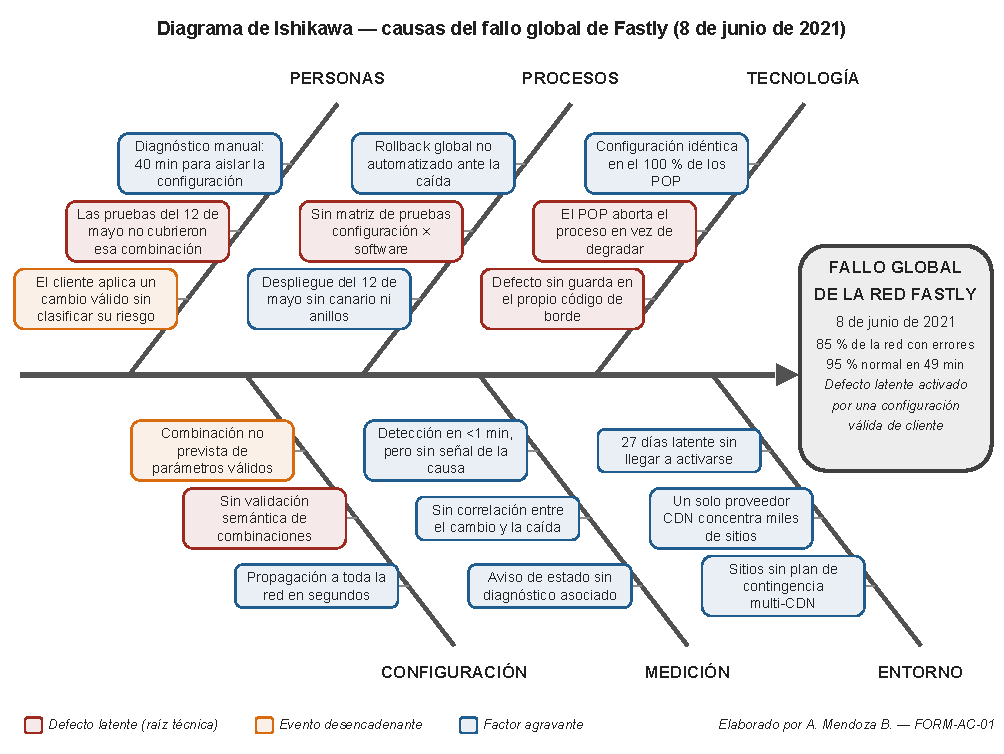
\includegraphics[width=\linewidth]{../diagramas/causas-fastly.pdf}
  \caption{Diagrama de Ishikawa del fallo del 8 de junio de 2021. Elaboración propia en
  draw.io; el archivo editable se conserva en \texttt{diagramas/causas-fastly.drawio}.}
  \label{fig:causas}
\end{figure}

\subsection*{Tres riesgos de SGIRI vinculados a estas causas}

\emph{SGIRI es el Sistema de Gestión de Incidencias que desarrollo como PFC: backend en Spring
Boot con PostgreSQL, frontend en Angular, tickets con estados y SLA, y adjuntos en Cloudinary.}

\begingroup
\small
\renewcommand{\arraystretch}{1.15}
\begin{tabularx}{\linewidth}{@{}YY@{}}
\toprule
Riesgo del PFC y consecuencia (categoría del diagrama) & Medida preventiva comprobable en TA-PFC-E1 \\
\midrule
\textbf{SGIRI:} un cambio válido en las reglas que mueven un ticket de un estado a otro (nuevo,
asignado, en proceso, resuelto, cerrado) puede dejarlo sin salida y con el reloj del SLA
corriendo (personas y procesos).
& Guardar cada versión de las reglas y probar todas las transiciones posibles antes de
activarlas; forzar una transición no permitida y comprobar que el ticket conserva su estado y
que el contador del SLA no salta. Validar la configuración al inicio es justamente lo que
falta en muchos sistemas~\cite[p.~619]{xu2016}. \\
\addlinespace
\textbf{SGIRI:} una versión nueva del backend con una credencial o una URL de base de datos mal
puesta no arranca y, al ser una sola instancia, el sistema entero queda caído (tecnología).
& Desplegar primero en un entorno de prueba, comprobar el arranque y la respuesta de salud
antes de pasar el tráfico, y conservar el paquete anterior para revertir. Tener copias no basta
si no se completa la cadena de detección, cambio y respaldo~\cite[p.~5]{gunawi2016}. \\
\addlinespace
\textbf{SGIRI:} los adjuntos dependen de Cloudinary; si el servicio externo falla o tarda, el
alta de la incidencia termina en error 500 y el ticket no se registra (entorno).
& Separar la subida del alta: guardar el ticket primero y subir el adjunto después, con tiempo
límite y reintento; comprobar con Cloudinary bloqueado que el ticket igual se registra. Lo
peor es abortar en vez de degradar~\cite[p.~250]{yuan2014}, y provocar el fallo a propósito es
la forma de verificarlo~\cite{basiri2016}. \\
\bottomrule
\end{tabularx}
\endgroup
